\documentclass{article}
\usepackage[utf8]{inputenc}
\usepackage[T1]{fontenc}
\usepackage[french]{babel}
\usepackage{graphicx}

\title{Rendu n.1 Projet technologique}
\author{Zoé Debaty}
\date{November 2019}

\begin{document}

\maketitle
\tableofcontents 
\newpage

% --------- Specificites techniques --------- %
\section{Spécificités techniques}

% --- L'image --- %
\subsection{Les images}
\subsubsection{Multicolor}
\begin{center} 
    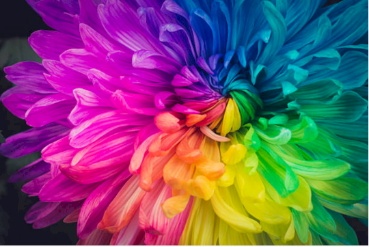
\includegraphics[width=9cm]{../Image_fonctions/Multicolor/Base.PNG}
\end{center}
\bigbreak

\begin{itemize}
\item Nom : "multicolor"
\item Dimensions : 612p * 408p
\item Taille : 59,9 Ko
\end{itemize}
\medbreak

L'image a été choisie car elle possède des changements de luminosité et énormément de couleurs afin de tester au mieux mes fonctions.

\subsubsection{Cat}
\begin{center} 
    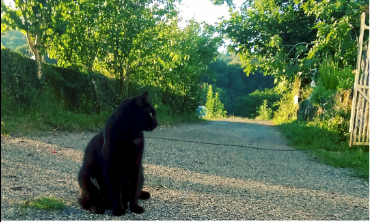
\includegraphics[width=9cm]{../Image_fonctions/Cat/Base.PNG}
\end{center}
\bigbreak

\begin{itemize}
\item Nom : "cat"
\item Dimensions : 1728p * 1036p
\item Taille : 1,87 Mo
\end{itemize}
\medbreak

Cette image est très grande et lourde et me permet de tester mes fonctions dans des cas extrèmes.

\subsubsection{Girl}
\begin{center} 
    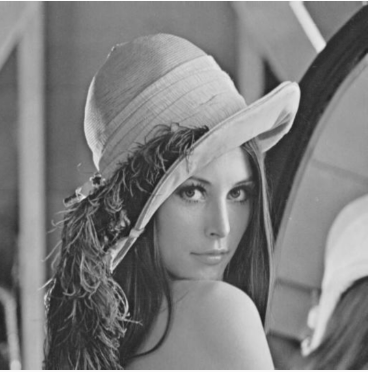
\includegraphics[width=9cm]{../Image_fonctions/Lenna/Base.PNG}
\end{center}
\bigbreak

\begin{itemize}
\item Nom : "Girl"
\item Dimensions : 512p * 512p
\item Taille : 31,4 Ko
\end{itemize}
\medbreak

Cette image est la plus légère et petite. Elle est de base en noir et blanc et est souvent utilisée en exemple dans les cours.
Elle me permet de tester facilement des fonctions de convolution.

% --- Le telephone --- %
\subsection{Le téléphone}
Pour tester mes fonctions j'utilise un Sony Xperia XA, avec un écran de 5 pouces.
Il tourne sous Android Nougat 7.0.

Toutes les performances ont été calculées sur ce téléphone. 
Les images ont été prises sur un émulateur Pixel 2 tournant sous Android 7.0.
\newpage

% ---------------- Fonctions ---------------- %
\section{Fonctions}

\subsection{TD_1 Introduction}
\subsubsection{Griser l'image}
\subsection{TD_3 Profilage de couleur}
\subsubsection{Coloriser l'image}
\subsubsection{Garder une couleur}
\subsection{TD_4 Contraste et Histogrammes}
\subsubsection{Extention de dynamique sur image grise}
\subsubsection{Extention de dynamique sur image couleur}
\subsubsection{Egalisation d'histogramme sur image grise}
\subsubsection{Egalisation d'histogramme sur image couleur}
\subsection{TD_5 Renderscript}
\subsubsection{Griser l'image}


\newpage
\section{Interface \underline{TD 3 Question 3.1}}
Pour l'interface, j'ai décidé d'avoir un menu défilant horizontal permettant d'avoir tout les boutons accessibles dans un espace reduit.
\bigbreak 

Pour les fonctions modifiant la saturation et la luminosité et pour la sélection de couleur, j'ai voulu
Je souhaiterais en finalité utiliser une "seekbar" afin d'avoir quelque chose de plus visuel pour l'utilisateur.
\bigbreak

Je me suis aussi rendue compte que mon application ne s’adaptait pas aux barres de navigation virtuelles (contrairement au Neffos qui possède des boutons physique). En effet, certains boutons étaient cachés par la barre. 
J'ai donc résolu ce problème en modifiant la visibilité de l'interface utilisateur au lancement de l'application. Mais si on verrouille l'application et qu'on retourne dessus, on peut voir que la barre fixe revient, ce sera donc un problème à régler.


\end{document}